\section{Einführung und das Paging-Problem}

\begin{takeaway}
    \item Online-Problem, Online-Algorithmus, kompetitiver Faktor
    \item Skirental-Problem
    \item Paging-Problem
    \item Randomisierte Online-Algorithmen
    \item Yaos Prinzip
\end{takeaway}

\paragraph{Motivation}
Probleme lösen und Entscheidungen fällen ohne alle für eine optimale Lösung relevanten Informationen zu haben.
Stattdessen werden die Informationen stückweise zur Laufzeit bekannt.

\paragraph{Beispiel: Skirental-Problem}
Unendlich langer Urlaub, nur an schönen Tagen Ski fahren.
Skier mieten für 1 CHF pro Tag, oder kaufen für $k$ CHF.
Erst am Tag selbst wird bekannt ob ein Tag schön ist.

Optimale Lösung: Sei $s$ die Anzahl schöner Tag.
Miete bei $s < k$, kaufe bei $s > k$, bei $s=k$ egal.

Problem: $s$ nicht bekannt, erst am Tag selber wird bekannt ob ein Tag schön ist.

\begin{table}[h]
    \begin{tabular}{l|l|c}
        Szenario & Worst Case & Approximationsgüte \\ \hline
        An Tag 1 kaufen & Ab Tag 2 schlechtes Wetter & $\frac{k}{1}$ \\
        Immer mieten & An $x >> k$ Tagen schönes Wetter & $\frac{x}{k}$ \\
        An $k-1$ Tagen mieten, dann kaufen & Ab Tag $k+1$ schlechtes Wetter & $\frac{2k-1}{k} = 2-\frac{1}{k}$
    \end{tabular}
\end{table}
\begin{figure}[h]
    \centering
    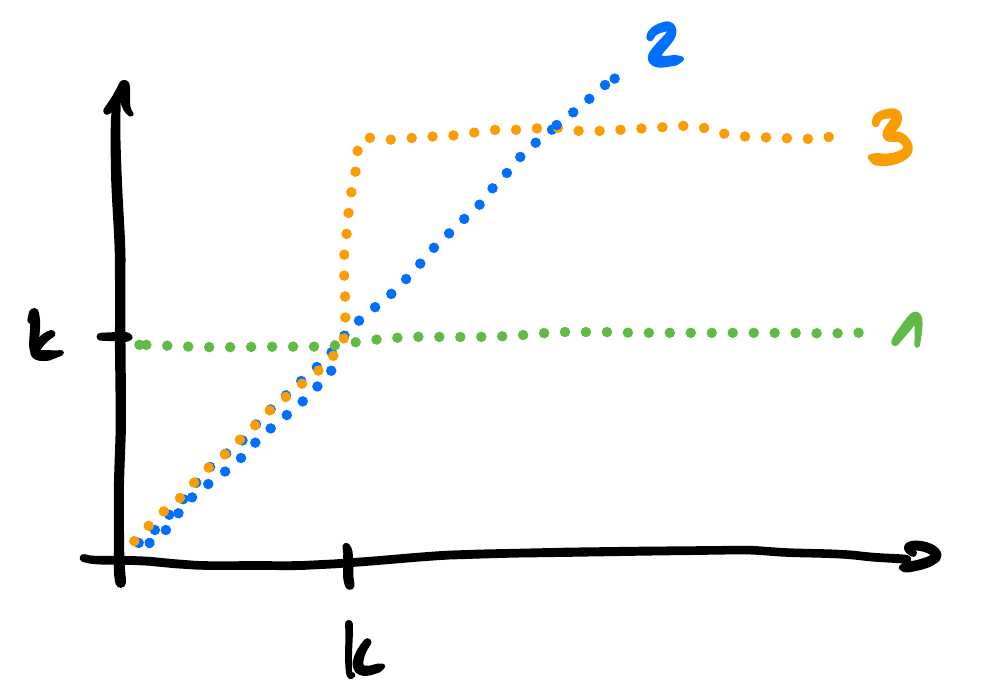
\includegraphics[width=0.3\textwidth]{images/skirental.png}
    \caption{Skirental Szenarios}
\end{figure}

\paragraph{Online-Problem}
Ein \emph{Online-Minimierungsproblem} ist $\Pi = (I, O, cost, \min)$.
Eine Eingabe $I = (x_1, ..., x_n) \in \mathcal{I}$ ist eine Folge von \emph{Anfragen},
jeweils für \emph{Zeitschritt} $i$.
Eine akzeptierte Lösung $O = (y_1, ..., y_n)$ ist eine Folge von \emph{Antworten}.

Beim analogen Maximierungsproblem spricht man statt von $cost(I, O)$ oft vom \emph{Gewinn} $gain(I,O)$.

\paragraph{Online-Algorithmus}
Sei $\Pi$ ein Online-Optimierungsproblem.
Ein \emph{Online-Algorithmus} $\A$ berechnet die Ausgabe $\A(I) = (y_1, ..., y_n) $
wobei $y_i$ nur von $(x_1, ..., x_i)$ abhängt.
$\A(I)$ ist eine zulässig Lösung für $I$.

\paragraph{Kompetitiver Faktor}
(aka. competitive ratio, Wettbewerbsgüte, kompetitive Güte) \\
Ein Online-Algorithmus $\A$ ist \emph{c-kompetitiv} falls gilt:
\begin{align*}
\exists \alpha \geq 0 \quad \forall I \cl \quad cost(\A(I)) & \leq c \cdot cost(Opt(I)) + \alpha \\
\dfrac{cost(\A(I))}{cost(Opt(I))} + \alpha' & \leq c
\end{align*}
für ein Minimierungsproblem und $\alpha$ konstant.
$Opt$ ist ein optimaler Offline-Algorithmus, d.h. mit vollständiger Information.

Für Maximierungsprobleme:
$$ gain(Opt(I)) \leq c \cdot gain(\A(I)) + \alpha $$

Das kleinste $c$ für das dies gilt heisst \emph{kompetitiver Faktor}. \\
$\A$ heisst \emph{strikt c-kompetitiv} falls $\alpha = 0$. \\
$\A$ heisst \emph{optimal} falls er strikt 1-kompetitiv ist ($\alpha = 0, c = 1$).

Wir sprechen hierbei von \emph{kompetitiver Analyse}.
Der kompetitiver Faktor ist vergleichbar mit der Approximationsgüte von Approximationsalgorithmen.

Ein Online-Algorithmus heisst \emph{kompetitiv} wenn sein kompetitiver Faktor nicht von der
Länge der Eingabe abhängt (d.h. es keine Startkosten gibt die amortisiert werden müssen).
Die Konstante $\alpha$ ist wichtig da sie erlaubt auf kurze Eingaben schlecht zu sein
(und erst auf lange besser zu werden).
\footnote{Warum brauchen wir bei der Approximationsgüte keine vergleichbare Konstante?}

\paragraph{Untere Schranken beweisen}
Für einen strikt kompetitiven Algorithmus:
Finde eine Instanz $I$ mit $\frac{\A(I)}{Opt(I)} > c$ $\implies$ \underline{nicht} strikt-kompetitiv.

Für einen nicht-strikt kompetitiven Algorithmus:
Finde eine unendliche Folge $I_1, I_2, ...$ von Instanzen so dass $\frac{\A(I_i)}{Opt(I_i)} > c$
und $Opt(I_i) \overset{i \rightarrow \infty}{\longrightarrow} \infty $.

\begin{figure}[h]
    \centering
    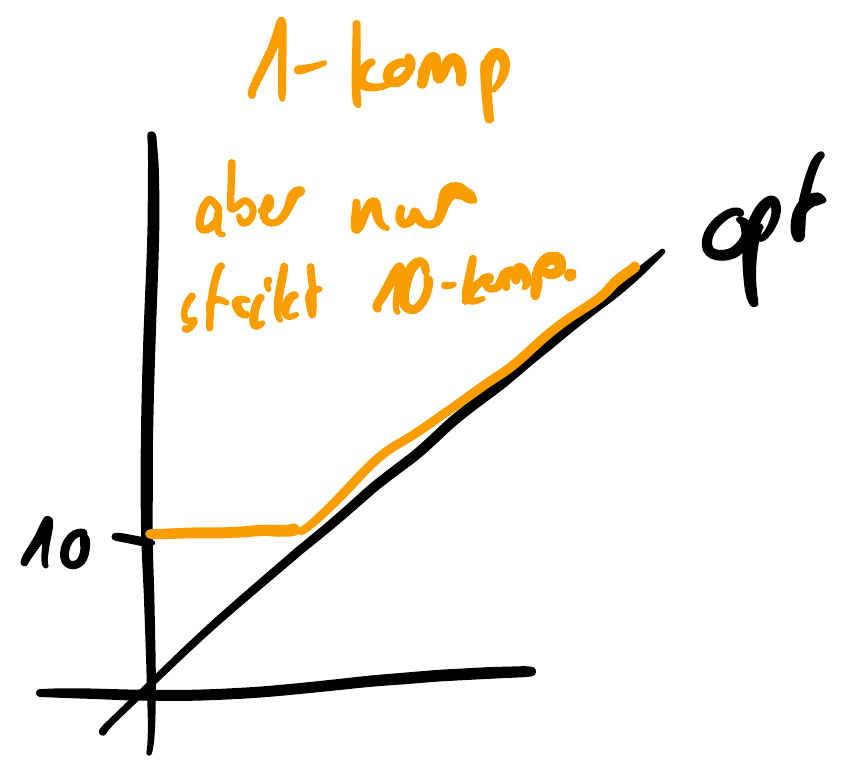
\includegraphics[width=0.2\textwidth]{images/strikt-kompetitiv.png}
    \caption{$Opt$ in schwarz. $\A$ in orange, 1-kompetitiv und strikt-10-kompetitiv.}
\end{figure}


\subsection{Das Paging-Problem}

\paragraph{Paging}
\begin{itemize}
    \item Eingabe: $ I = (x_1, ..., x_n)$ mit Speicher-Indizes $x_i \in \N$
    \item Hauptspeicher mit $m$ Seiten: $ (s_1, ..., s_m) $
    \item Cache-Speicher mit $k$ Seiten: $ B = (s_{j_1}, ..., s_{j_k}) $, initialisiert mit $ (s_1, ..., s_k) $
        \footnote{Der Vorsprung eines selbstgewählten Startinhalts kann in $\alpha$ versteckt werden.}
    \item Zeitschritt $i$:
    \begin{itemize}
        \item Index $x_i$ wird angefragt
        \item Falls $x_i$ im Cache (d.h. $s_{x_i} \in B$): return $y_i=0$
        \item Andernfalls: return $y_i=j$, und setze $B = B \backslash  \{s_j\} \cup \{s_{x_i}\} $,
            d.h. lösche Seite $s_j$ aus dem Cache und ersetze sie durch $s_{x_i}$.
            \footnote{Zusätzliches, proaktives Entfernen bringt keinen Vorteil.}
    \end{itemize}
    \item $ cost(\A(I)) := \vert \{ i \st y_i > 0 \} \vert $
    \item goal := min
\end{itemize}

Strategien bei \emph{Seitenfehlern (page faults)} zum \emph{Verdrängen} von Seiten:
First-in-First-Out (FIFO, wie eine Queue),
Last-in-First-Out (LIFO, wie ein Stack),
Least-Recently-Used (LRU),
Longest-Forward-Distance (LFD, offline-only!).

\paragraph{Satz (FIFO)}
Ein Online-Algorithmus für Paging der FIFO nutzt ist strikt-k-kompetitiv.

\underline{Beweis:}
Gruppiere Zeitschritte in \emph{Phasen}.
Phase 1 endet nach dem ersten Seitenfehler.
Phase $P \geq 2$ endet nach $1+ (P-1)k$ Seitenfehlern, d.h. alle $k$ Fehler endet eine Phase und beginnt eine neue.

In Phase 1 machen $Opt$ und $Fifo$ je genau einen Fehler (warum?).

Sei $s$ die Seite die den letzten Seitenfehler von Phase $P-1$ verursacht
(d.h. sie kommt neu in den Cache, und wird dank FIFO als letztes in Phase $P$ verdrängt werden). \\
$\implies$ Zu Beginn von Phase $P$ ist $s$ im Cache von $Opt$ \underline{und} von $Fifo$. \\
$\implies$ Es gibt $\leq k-1$ Seiten die im Cache von $Opt$ sind, aber nicht in dem von $Fifo$. \\
Während Phase $P$ macht $Fifo$ genau $k$ Fehler. \\
$\implies$  Während $P$ muss $Opt$ mindestens einen Seitenfehler machen. \\
$\implies$  $Fifo$ ist k-kompetitiv.

LRU ist in der Theorie ebenfalls k-kompetitiv, in der Praxis allerdings tendenziell besser als FIFO.

\paragraph{Satz (untere Schranke)}
Kein Online-Algorithmus für Paging kann eine besseren kompetitiven Faktor als k erreichen.

\underline{Beweis:}
Sei $k$ die Grösse vom Cache und $k+1$ die Grösse vom Hauptspeicher.
\footnote{$k+1$ macht die Aussage nur stärker. Warum?}
Betrachte die "worst case" Eingabe $ I = (k+1, s_{y_1}, s_{y_2},, ..., s_{y_{n-1}}) $,
d.h. in Zeitschritt $i$ wird die Seite angefragt die $\A$ zuvor erst verdrängt hat.
$\A$ verursacht also exakt $k$ Seitenfehler, und $Opt$ nur einen in Zeitschritt 1.

\underline{Für alle Strategien} von $\A$ lässt sich eine worst-case Eingabe konstruieren (siehe Idee
eines \emph{Gegenspielers} der die Strategie/den Quellcode kennt).
Durch Wiederholen solcher k-langen Phasen lässt sich ausserdem eine \underline{unendlich lange}
Eingabe konstruieren.
Eingabelänge $n$, $\A$ mit $n$ Fehlern, $Opt$ mit $n/k$ Fehlern $\implies$ k-kompetitiv.
\footnote{Mit etwas Glück (abhängig davon was $\A$ in zukünftigen Phasen verdrängt)
macht $Opt$ sogar nur den Fehler in Zeitschritt 1, und macht danach nie wieder einen Fehler.}


\subsection{Randomisierte Online-Algorithmen}

\paragraph{Motivation}
Randomisierung verunmöglicht es dem Gegenspieler die genaue Strategie von $\A$ zu kennen,
d.h. es verunmöglicht ihm eine worst case Instanz zu konstruieren.

\paragraph{Randomisierter Online-Algorithmus}
Bekommt als Eingabe zusätzlich ein unendliche langes Zufallsband $\phi$ mit Zufallsbits
(die u.a.r. 0 oder 1 sind).
Jede Antwort $y_i$ darf nur von $ \phi, x_1, ..., x_i, y_1, ..., y_{i-1} $ abhängen.

\underline{Beobachtung:}
Jeder randomisierte Algorithmus $Rand$ der $b(n)$ Zufallsbits für Eingaben der Länge $n$ liest
kann als eine Menge $ strat(Rand) = \{ A_1, ..., A_{2^{b(n)}} \} $ von $2^{b(n)}$ deterministischen
Online-Algorithmen angesehen werden, von denen einer mit Wahrscheinlichkeit jeweils $\frac{1}{2^{b(n)}}$
ausgewählt wird.

\paragraph{Erwarteter kompetitiver Faktor}
Ein Online-Algorithmus $Rand$ ist \emph{c-kompetitiv im Erwartungswert} falls
$$ \exists \alpha \geq 0 \quad \forall I \cl \quad
\mathbb{E} [ cost(Rand(I)) ] \leq c \cdot cost(Opt(I)) + \alpha $$

Das kleinste $c$ für das dies gilt heisst \emph{erwarteter kompetitiver Faktor}. \\
$Rand$ heisst \emph{strikt c-kompetitiv im Erwartungswert} falls $\alpha = 0$.

\paragraph{Wahrscheinlichkeitsverstärkung}
Einen randomisierten Offline-Algorithmus der mit Wahrscheinlichkeit $\frac{1}{2}$ korrekt ist,
kann man $k$ Mal wiederholen um $\frac{1}{2^k}$ zu erreichen.
Online ist dies \underline{nicht} möglich, da wir direkt eine Antwort auf jede Anfrage geben müssen.

\paragraph{Randomisierter Paging-Algorithmus RMark}
Eine Phase endet/beginnt wenn nach einem Seitenfehler alle Seiten unmarkiert werden.

\begin{algorithm}[h]
\caption{RMark}
\begin{algorithmic}
    \State mark alle Seiten im Cache
    \While{Eingabe ist noch nicht beendet}
        \State $s \gets$ Seite mit Index $x_i$
        \If{$s$ ist im Cache}
            \If{$s$ ist unmarkiert}
                \State mark $s$
            \EndIf
        \State output "0"
        \Else
            \If{es existiert keine unmarkierte Seite mehr im Cache}
                \State unmark alle Seiten im Cache
            \EndIf
            \State $s' \gets$ zufällig gewählte unmarkierte Seite
            \State verdränge $s'$ und füge $s$ an der alten Stelle von $s'$ ein
            \State mark $s$
            \State output "Index von $s'$ "
        \EndIf
    \State $i \gets i + 1$
    \EndWhile
\end{algorithmic}
\end{algorithm}


\paragraph{Satz}
$RMark$ hat einen erwarteten kompetitiven Faktor von $2 H_k$.
\footnote{Für jedes $l \in \N^+$ heisst $H_l$ die \emph{l-te Harmonische Zahl}
und $H_l := 1 + \frac{1}{2} + \frac{1}{3} + \dots + \frac{1}{l} = \sum_{i=1}^l \frac{1}{i} $.}
D.h. $RMark$ ist im Erwartungswert $\bigO(\log k)$-kompetitiv.

\underline{Beweis:} Siehe auch Skript S.14ff.

Betrachte eine einzelne Phase $P$.
O.B.d.A werden $k$ veschiedene Seiten angefragt (eventuell auch mehrmals).
Im worst case werden zuerst $l$ "neue" Seiten angefragt, und danach $k-l$ "alte".
Mit Wahrscheinlichkeit $(k-l)/k$ ist die erste alte Seite noch im Cache,
dann mit Wahrscheinlichkeit $(k-l-1)/(k-1)$ die zweite alte, usw.
Umgekehrt ist die $i$-te alte Seite mit Wahrscheinlichkeit
$1 - \frac{k-l-(i-1)}{k-(i-1)} = \frac{l}{k-(i-1)}$ \underline{nicht} mehr im Cache.
Die erwarteten Kosten während $P$ sind also
$$ l + \sum_{i=1}^{k-l} \dfrac{l}{k-(i-1)} = \dots = l (H_k - H_l +1) \leq l H_k $$
Ausserdem gilt $l \geq 1$ da jede Phase per Definition mit einer neuen Seite beginnt.

Betrachte die Kosten von $Opt$.
Betrachte zwei aufeinanderfolgende Phasen $P_{j-1}, P_j$.
In diesen wurden $\geq k+l_j$ verschiedene Seiten angefragt.
$\implies$ $Opt$ macht $\geq l_j$ Seitenfehler.
$RMark$ und $Opt$ machen in $P_1$ beide $l_1$ Fehler (da sie mit demselben Cache starten).

Durch unterschiedliches Gruppieren ($(P_1, P_2), (P_3, P_4), ...$ vs $P_1, (P_2, P_3), (P_4, P_5), ...$)
erhalten wir:
$$ cost(Opt(I))
    \geq \max \left\{ \sum_{i=1}^{ \lfloor N/2 \rfloor } l_{2i} , \sum_{i=1}^{ \lceil N/2 \rceil } l_{2i-1} \right\}
    \geq \frac{1}{2} \left( \sum_{i=1}^{ \lfloor N/2 \rfloor } l_{2i} + \sum_{i=1}^{ \lceil N/2 \rceil } l_{2i-1} \right)
    = \sum_{i=1}^{N} \frac{1}{2} l_i
$$

Der kompetitive Faktor ist also
$$ c \geq \dfrac{ \sum_{i=1}^{N} H_k l_i }{ \sum_{i=1}^{N} \frac{1}{2} l_i } = 2 H_k $$

\paragraph{Verbesserung}
Für Paging existiert kein deterministischer Online-Algorithmus mit kompetitivem Faktor $k$ (s.o.).
Mit Randomisierung können wir im Erwartungswert aber $\bigO(\log k)$ erreichen!
D.h. asymptotisch expontentieller Speedup!
Dies ist asymptotisch optimal für randomisierte Algorithmen (s.u.).


\subsection{Yaos Prinzip}

\paragraph{Motivation}
Untere Schranke für kompetitiven Faktor von deterministischen OAs
$\implies$ Untere Schranke für erwarteten kompetitiven Faktor von randomisierten OAs

Wahrscheinlichkeitsverteilung über Instanzen $\Pr_{Adv}$ $\implies$ W'keitsverteilung über Algorithmen $\Pr_{Rand}$.

Limitierung: konstante Anzahl von Instanzen $\I = \{I_1, ..., I_m\}$ und Algorithmen
$strat(Rand) = \{A_1, ..., A_l\}$ (d.h. Eingabelänge $n$ begrenzt).

\paragraph{Lemma 1 (1.13)}
Sei $\Pi$ ein Optimierungsproblem, sei $\I$ eine Klasse von Instanzen.
Sei $\Pr_{Adv}$ eine W'keitsverteilung so dass gilt:
$$ \forall A \in strat(Rand) \cl \E_{Adv}[cost(A(\mathsf{I}))] \geq c \cdot \E_{Adv}[cost(Opt(\mathsf{I}))] $$
Dann gilt:
$$ \forall Rand \; \exists I \in \I \cl \E_{Rand}[cost(\mathsf{A}(I)))] \geq c \cdot cost(Opt(I)) $$
wobei $\mathsf{A} ,\mathsf{I}$ Zufallsvariablen sind aus den Wahrscheinlichkeitsräumen $\Pr_{Rand}, \Pr_{Adv}$.

\underline{Beweis:} Siehe Skript S.18f.

\paragraph{Lemma 2 (1.14)}
Seien $\Pi, \I, \Pr_{Adv}$ wie oben.
Sei $\forall$ det. OAs $A_j$ der erwartete kompetitive Faktor $\geq c$, d.h.
$$ \E_{Adv} \left[ \dfrac{cost(A_j(\mathsf{I}))}{cost(Opt(\mathsf{I}))} \right] \geq c $$

Dann gilt:
$\forall$ rand. OAs ist der erwartete kompetitive Faktor $\geq c$, d.h. $\exists I \in \I$ so dass
$$ \dfrac{ \E_{Rand} [ cost(\mathsf{A}(I)) ]}{cost(Opt(I))} \geq c $$

\underline{Beweis:} Siehe Skript S.20f.

\paragraph{Satz (Yaos Prinzip)}
Folgt aus Lemma 1 und 2.
Seien $\Pi, \I, \Pr_{Adv}$ wie oben.
Für jeden randomisierten Online-Algorithmus existiert dann eine Eingabe $I$ so dass
$$
\dfrac{\E_{Rand}[cost(\mathsf{A}(I))]}{cost(Opt(I))}
    \geq \max \left\lbrace
    \left\lbrace \min_j \dfrac{\E_{Adv}[cost(A_j(\mathsf{I}))]}{\E_{Adv}[cost(Opt(\mathsf{I}))]} \right\rbrace,
    \left\lbrace \min_j \E_{Adv} \left[ \dfrac{cost(A_j(\mathsf{I}))}{cost(Opt(\mathsf{I}))} \right] \right\rbrace
    \right\rbrace
$$

Anders formuliert (laut Wikipedia):
$$ \max_{I \in \I} \E_{Rand}[cost(\mathsf{A}(I))] \geq \min_{A \in strat(Rand)} \E_{Adv}[cost(A(\mathsf{I} ))] $$
wobei $\mathsf{A}, \mathsf{I}$ Zufallsvariablen sind.

\paragraph{Spieltheoretische Interpretation}
Yaos Minimax Prinzip. Spezialfall von Von Neumanns Minimax Theorem (in Nullsummenspielen mit
2 Spielern und gemischten Strategien gibt es ein Gleichgewicht).
Zero-sum game, Spieler A wählt den det. Algorithmus, Spieler B wählt die Instanz, der payoff ist $cost(A_j(I))$.

Für jeden Spieler ist "zufällig wählen" eine Strategie.
Aus Yao folgt: für eine fixe Eingabe zufällig eine Algo wählen ist nicht schlechter
als für einen fixen Algo zufällig eine Eingabe wählen.

\paragraph{Satz (Untere Schranke für randomisiertes Paging)}
Kein randomisierter Online-Algorithmus für Paging kann einen besseren (= kleineren) erwarteten
kompetitiven Faktor als $H_k$ erreichen.

\underline{Beweis:}
Siehe Skript S.27ff.

Analog zu Paging: $k$ Cache, $k+1$ Hauptspeicher, frage zuerst $s_{k+1}$ an, danach (neu!) jede
der nicht gerade angefragten Seiten mit Wahrscheinlichkeit $\frac{1}{k}$.
Eine Phase endet nach $k$ Fehlern, d.h. nachdem alle $k+1$ Seiten mind. einmal angefragt wurden.

Betrachte einzelne Phase. Zeige dass für alle deterministischen  $A_j$ die erwarteten Kosten circa
\mbox{$H_k$-mal} höher sind als die von $Opt$.
Es gilt für die Eingabe während Phase $P$:
$$ \dfrac{\E_{Adv} [cost(A_j(P))]}{\E_{Adv} [cost(Opt(P))]} \geq \dfrac{|P|\cdot \frac{1}{k}}{1} = \dfrac{|P|}{k} $$

Schätze ab (siehe Skript, siehe Coupon Collector): $\quad \E_{Adv}[\,|P|\,] = 1 + k \cdot H_k$.

Wende Yaos Prinzip an:
$$ \dfrac{\E_{Rand}[cost(\mathsf{A}(I))]}{cost(Opt(I))} \geq H_k $$
